\documentclass[11pt, oneside]{article}   	% use "amsart" instead of "article" for AMSLaTeX format
\usepackage{geometry}                		% See geometry.pdf to learn the layout options. There are lots.
\geometry{letterpaper}                   		% ... or a4paper or a5paper or ... 
%\geometry{landscape}                		% Activate for for rotated page geometry
%\usepackage[parfill]{parskip}    		% Activate to begin paragraphs with an empty line rather than an indent
\usepackage{graphicx}				% Use pdf, png, jpg, or eps§ with pdflatex; use eps in DVI mode
								% TeX will automatically convert eps --> pdf in pdflatex		
\usepackage{amssymb}

\title{Fashion data set analysis}
\author{Sabrina Yue Wang}
%\date{}							% Activate to display a given date or no date

\begin{document}
\maketitle
\section{Introduction and plan}
The implementation utilises the sklearn python package which has inbuilt classifiers, those of which are tested are support vector machines and random forest models. The important thing to note that comparison between different classifiers is not as important as the preprocessing of the data to maximise the differences between the classes for easier distinguishability. Initially, the matrices for all the training datasets were naively  put into the sklearn.svm.NuSVR classifier took almost a day. This is unrealistic and thus the main part of the code looks at a simple linear variable reduction analysis.

\section{PCA and LDA Implementation and results}
Sebastian Raschka provides simple examples of Principle component analysis (PCA) \cite{PCA} and Linear disciminant analysis (LDA) \cite{LDA} from which the code is adapted from. PCA is used to map the data onto a different subspace, often with lower dimensions. The effectiveness of this method depends on the magnitude ratios between the eigenvalues of the scatter matrix, a method of approximating the covariance matrix which is a generalisation of the variance for higher dimensions. If the largest eigenvalues are much larger than the rest, then it is 'safer' to neglect the smaller eigenvalues (and their corresponding eigenvectors). Once the eigenvalues and vectors are determined the training set can be mapped onto the new subspace using the eigenvectors. This reduction in complexity as well as method of separating properties amongst the total dataset increases the speed and accuracy of classifiers implemented on the transformed input data. Multiple Discriminant analysis is a similar method of separating features, except it is more concerned with the variance between different classes rather than the whole dataset. Both methods are implemented (see fashion.py).

The analyse function in fashion.py returns the score when the trained estimator (final one settled on was sklearn.ensemble.ExtraTreesClassifier()) is applied on the test data (which is transformed like the PCA and LDA testing sets and then scaled). Finally, the effects of the number of largest eigenvalues used on the classifier is investigated through a scan of the k's used in the PCA and LDA. The best possible resulting score from the analysis came out to be $\approx 0.71$, when the kdim=kLDA=11 (NB they were not varied individually as it would take too long so this is estimate of best values. Also the number 12 can fluctuate between 9 and 12 as these values produce similar results). The whole program should run in approximately 6 minutes and the plots for the best choice of the number of eigenvalues used for PCA/LDA is shown in Figure \ref{fig:fig1}, whereas the terminal outputs will be something similar to Figure \ref{fig:fig2}:

\begin{figure}[H]
\centering
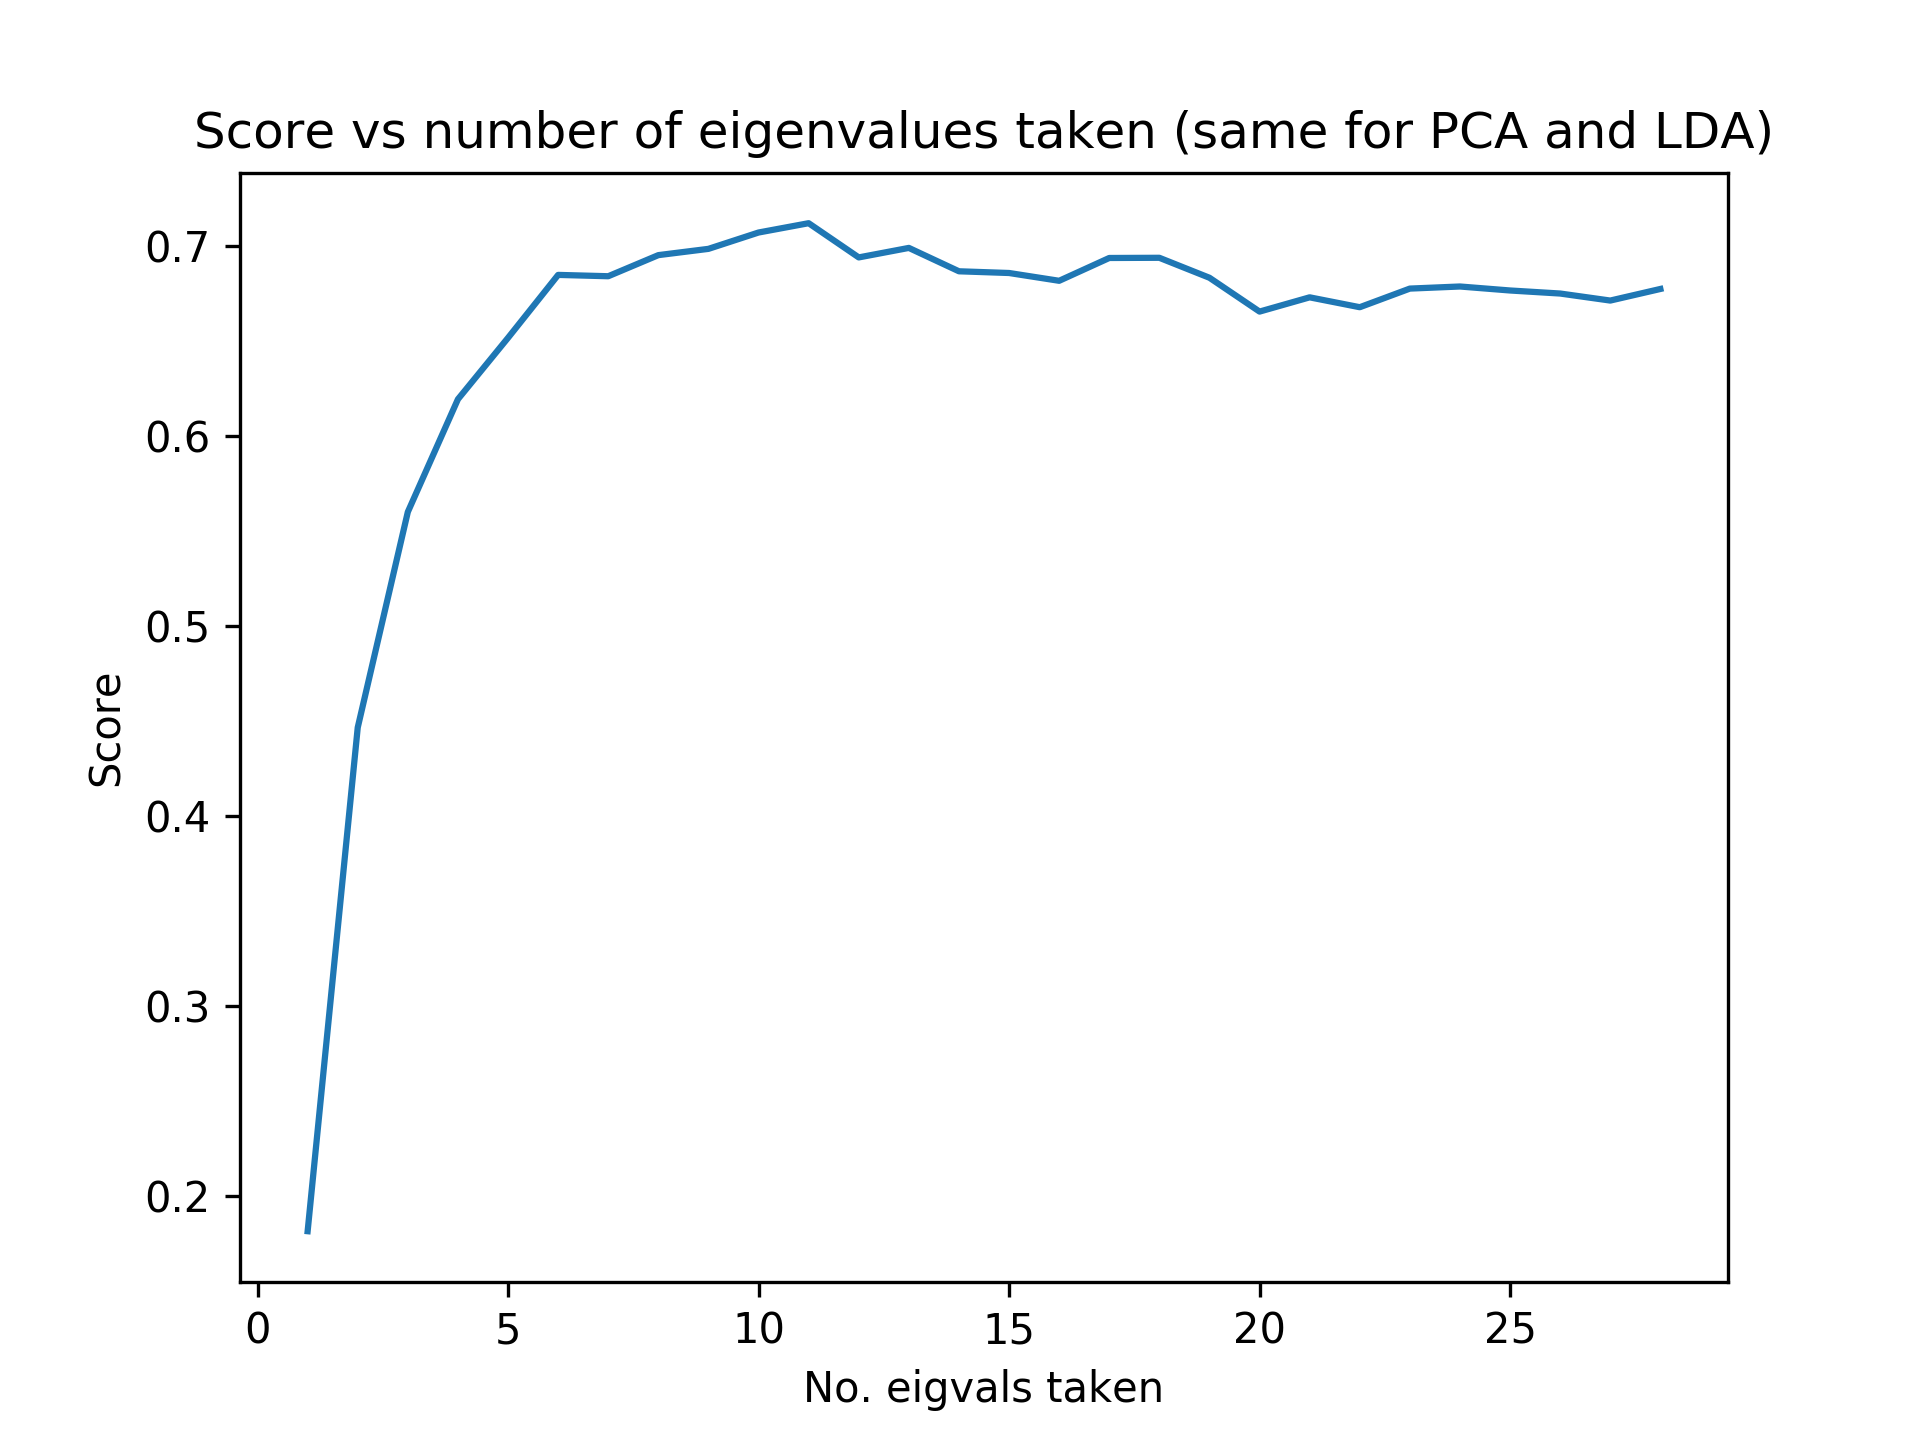
\includegraphics[scale=0.7]{pythonfileoutput.png}
\label{fig:fig1}
\caption{Python file fashion.py output figure: showing that if the number of eigenvalues used for PCA and LDA are taken to be the same then the best value is around 9-12 (usually 12)}
\end{figure}
\begin{figure}[H]
\centering
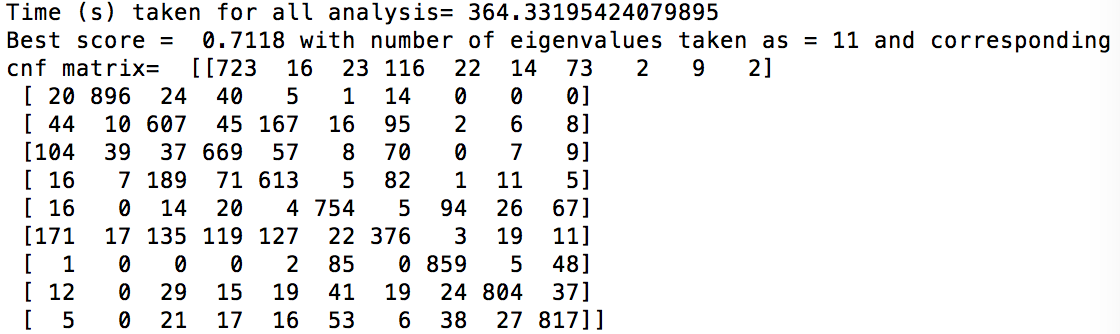
\includegraphics[scale=0.7]{terminaloutput.png}
\label{fig:fig2}
\caption{Terminal output when kdim=kLDA=12, using the ExtraTreesClassifier, showing the score and corresponding confusion matrix when predicting on the xtest and ytest datasets.}
\end{figure}


Notes on the code that is commented out:
\begin{itemize}
\item lines 67-166 show that the confusion matrix (using svm.NuSVR) after almost a day of running turned out very inaccurate (please don't run it)
\item Lines 201-205 and 356-360 are commented out because instead of taking the mean of each row of the input matrices before applying PCA and LDA, the vector of eigenvalues are calculated and used in the analysis instead, which gave worse prediction scores.
\item Lines 292-298 is a quick plot showing the visual differences between the first 2 classes in the dictionary after PCA and LDA is applied.
\item Lines 317-338 uses a KFold split ($n\_splits$ is self chosen) such that the cross validation method reveals how the classifier does against the data (i.e. the performance of the chosen classifier). It takes a few (2-3) minutes to run, outputting a score and confusion matrix. Note that the number of splits (used in KFold) can slightly change the outcome of how the perform seems to be. Too large of a split means that the number of combinations of each group is less, so avoid that. However, in the end when the fitting is done for the dataset this is neglected. 
\item lines 375-380 plots the average vector values of the first image of every class, showing they are quite different. Lines 381-393 plots the first N pictures of a few classes, showing large variation within the classes and thus there is a lot of overlap.
\end{itemize}

\section{Other classification methods and future improvements}
The random forest model is used for the classification as it is faster in speed compared to support vector machine models. In order to further improve the classifier, one can use other non-linear classification methods with non linear kernels, for example using deep learning methods with different layers (e.g. neural networks which sklearn does have inbuilt but sadly I didn't spend enough time studying it in the break :( ) as they have methods of feature extraction (e.g. some pictures may have sharper changes in curvature) that can help increase the distinguishability of class features. Finally for the preprocessing phase, there are fractal methods which make use of fractal characteristics (e.g. fractal dimension) of the data and thus lead to picking out characteristics of data sets that are similar/hard to distinguish using the naked eye. However, this method often will enhance characteristics both between and within classes, improving and damaging the effectiveness of preprocessing respectively. Furthermore fractal methods usually are applied to  data that has a lot of details such as market fluctuations and natural phenomena, which is not really applicable here but may be interesting to try out and see which effect dominates.

\bibliographystyle{ieeetr}
\bibliography{Master}
NB: The url does not seem to work when I use bibtex so please either google Sebastian Raschka and the title of the page or copy the link by hand. Sorry for the inconvenience.
\end{document}  